\documentclass[12pt,a4paper]{article}
\usepackage[utf8]{inputenc}
\usepackage[T1]{fontenc}
\usepackage[spanish,es-tabla]{babel}
\usepackage[margin=2.5cm]{geometry}
\usepackage{graphicx}
\graphicspath{{./}}
\usepackage{booktabs}
\usepackage{tabularx}
\usepackage{array}
\usepackage{longtable}
\usepackage{hyperref}
\usepackage{amsmath}
\usepackage{cite}
\usepackage{fancyhdr}
\usepackage{enumitem}

\hypersetup{colorlinks=true,linkcolor=black,citecolor=black,urlcolor=blue}
\setlength{\parskip}{0.45em}
\setlength{\parindent}{1.25cm}
\renewcommand{\arraystretch}{1.25}

\pagestyle{fancy}
\fancyhf{}
\rhead{Ingeniería de Requerimientos - UTEQ}
\lhead{TA-IND-01: Chess.com}
\rfoot{Página \thepage}

\begin{document}

\begin{titlepage}
    \centering
    {\scshape\LARGE Universidad Técnica Estatal de Quevedo \par}
    {\scshape\Large Facultad de Ciencias de la Ingeniería\par}
    {\scshape\large Carrera de Ingeniería en Software\par}
    \vspace{1.5cm}
    {\huge\bfseries TA-TAR-01 - SUM - Trabajo individual: IEEE 29148 y tipos de requisitos de un sistema conocido\par}
    \vspace{1cm}
    {\Large\itshape Autor: Jordy Rivas Bodero\par}
    {\Large Asignatura: Ingeniería de Requerimientos\par}
    \vfill
    {\large Fecha de entrega: 7 de noviembre de 2026\par}
\end{titlepage}

\renewcommand{\contentsname}{Índice}
\clearpage
\tableofcontents
\clearpage

\section{Resumen analítico de la norma ISO/IEC/IEEE 29148:2018}

La norma ISO/IEC/IEEE 29148:2018 establece lineamientos para desarrollar, documentar y gestionar requisitos durante el ciclo de vida de un sistema o producto de software. Su propósito es que las necesidades de las partes interesadas se conviertan en requisitos claros, coherentes y que puedan comprobarse. Esto es importante porque una descripción imprecisa puede provocar que el equipo de desarrollo interprete una función de una manera distinta a la que espera el usuario. En consecuencia, los requisitos no deben limitarse a expresar ideas generales: tienen que describir condiciones o capacidades concretas del sistema \cite{ieee29148}.

\subsection{Requisito bien formado (cláusula 5.2.4)}

De acuerdo con la cláusula 5.2.4, un requisito bien formado expresa una necesidad o condición que debe cumplir el sistema y está redactado de manera que pueda entenderse y verificarse. Para conseguirlo, debe identificar con claridad el sujeto al que se refiere, la condición o capacidad esperada y, cuando corresponda, las restricciones que delimitan su cumplimiento. También debe evitar reunir varias obligaciones independientes en una sola oración.

Por ejemplo, decir que ``Chess.com debe funcionar rápidamente'' no permite determinar cuándo se considera que el sistema cumple. En cambio, indicar que ``el sistema debe reflejar el movimiento realizado por un jugador en el tablero de su oponente en un máximo de 150 milisegundos, bajo las condiciones de prueba establecidas'' presenta una condición que puede medirse. La diferencia está en que el segundo enunciado permite preparar una prueba y comparar el resultado con un umbral definido.

\subsection{Características de un requisito individual (cláusula 5.2.5)}

La cláusula 5.2.5 establece características que permiten evaluar la calidad de cada requisito. Aplicadas al caso de Chess.com, se pueden explicar de la siguiente manera:

\begin{itemize}[leftmargin=*]
    \item \textbf{Necesario:} responde a una necesidad real de una parte interesada o a una obligación del sistema. Por ejemplo, registrar los movimientos de una partida es necesario para que el usuario pueda revisar su desarrollo.
    \item \textbf{Apropiado:} expresa el nivel de detalle adecuado para el elemento del sistema al que se dirige, sin imponer soluciones innecesarias.
    \item \textbf{Inequívoco:} tiene una sola interpretación razonable. Expresiones como ``muy rápido'' o ``fácil de usar'' deben sustituirse por condiciones precisas.
    \item \textbf{Completo:} contiene la información necesaria para comprender qué se espera, sin depender de explicaciones que no estén incluidas o referenciadas.
    \item \textbf{Singular:} expresa una sola obligación. Por ejemplo, emparejar jugadores y actualizar sus puntuaciones deben redactarse como requisitos separados.
    \item \textbf{Factible:} puede implementarse teniendo en cuenta los recursos, la tecnología, el tiempo y las restricciones del proyecto.
    \item \textbf{Verificable:} permite comprobar su cumplimiento mediante pruebas, inspecciones, análisis o demostraciones.
    \item \textbf{Correcto:} representa fielmente la necesidad de la que procede y no introduce condiciones equivocadas.
    \item \textbf{Conforme:} respeta la estructura y las reglas de redacción establecidas para documentar los requisitos.
\end{itemize}

Estas características ayudan a evitar que un requisito dependa de la interpretación personal de quien lo desarrolla o evalúa. Además, facilitan la comunicación entre usuarios, analistas, programadores y responsables de las pruebas.

\subsection{Características del conjunto de requisitos (cláusula 5.2.6)}

No basta con que cada requisito esté bien redactado de manera individual. El conjunto también debe representar de forma ordenada las necesidades del sistema. Según la cláusula 5.2.6, se debe revisar que los requisitos estén completos, sean consistentes y mantengan relaciones comprensibles entre sí. En el caso de Chess.com, por ejemplo, las reglas de emparejamiento no deberían contradecir las condiciones que determinan el inicio de una partida.

También es importante que el conjunto sea viable, necesario y trazable. La trazabilidad permite relacionar cada requisito con su origen, su diseño y las pruebas que comprobarán su cumplimiento. Por su parte, la posibilidad de modificar los requisitos de forma controlada ayuda a gestionar cambios sin generar contradicciones en otras partes del sistema. En conjunto, estas características permiten que el documento funcione como una referencia durante el desarrollo y no solamente como una lista de funciones.

\subsection{Expresiones ambiguas que deben evitarse}

En la redacción de requisitos conviene evitar palabras cuyo significado dependa de la opinión de cada persona. Algunos ejemplos son ``rápido'', ``intuitivo'', ``eficiente'', ``amigable'', ``seguro'', ``fácil'' o ``adecuado''. Estas expresiones no siempre son incorrectas en una conversación inicial, pero no son suficientes para establecer por sí solas un criterio de aceptación.

En lugar de escribir que una partida debe desarrollarse de forma ``fluida'', se puede definir un tiempo máximo de respuesta y las condiciones en las que se medirá. De igual manera, en lugar de indicar que la plataforma debe ser ``segura'', se debe especificar qué controles se esperan, como el almacenamiento de contraseñas mediante funciones de derivación de claves adecuadas. La intención no es eliminar el lenguaje cotidiano de todo el proyecto, sino convertir las expectativas generales en condiciones concretas cuando se documenten como requisitos.

\section{Glosario de términos (cláusula 3)}

A continuación se presentan diez términos relacionados con la cláusula 3 de la norma ISO/IEC/IEEE 29148:2018. Cada definición se acompaña de un ejemplo aplicado a Chess.com.

\begin{enumerate}[leftmargin=*]
    \item \textbf{Requisito (Requirement):} necesidad o condición que debe cumplir un sistema, producto o servicio. \textit{Ejemplo:} Chess.com debe registrar los movimientos válidos realizados durante una partida.
    \item \textbf{Parte interesada (Stakeholder):} persona u organización que puede afectar al sistema, verse afectada por él o tener interés en sus resultados. \textit{Ejemplo:} los jugadores, moderadores y organizadores de torneos que utilizan la plataforma.
    \item \textbf{Línea base (Baseline):} versión aprobada de un conjunto de elementos que sirve como referencia para controlar cambios. \textit{Ejemplo:} la versión aprobada de los requisitos del módulo de partidas antes de iniciar su implementación.
    \item \textbf{Verificación (Verification):} actividad que comprueba si un producto o resultado cumple los requisitos especificados. \textit{Ejemplo:} ejecutar pruebas para comprobar que el sistema rechaza un movimiento ilegal de una pieza.
    \item \textbf{Validación (Validation):} actividad que determina si el sistema o producto satisface las necesidades de sus usuarios en el contexto previsto. \textit{Ejemplo:} realizar una prueba con jugadores para comprobar que pueden iniciar y completar una partida sin dificultades que impidan su uso.
    \item \textbf{Concepto de operación (ConOps):} descripción de cómo se espera que un sistema sea utilizado y opere desde la perspectiva de sus usuarios y partes interesadas. \textit{Ejemplo:} describir cómo un jugador inicia sesión, busca un oponente, juega una partida y consulta sus resultados.
    \item \textbf{Interfaz (Interface):} límite compartido mediante el cual interactúan dos sistemas, componentes o elementos. \textit{Ejemplo:} la interfaz de comunicación entre el navegador del jugador y los servicios que gestionan la partida.
    \item \textbf{Trazabilidad (Traceability):} posibilidad de relacionar un requisito con su origen y con los elementos que se derivan de él. \textit{Ejemplo:} vincular el requisito de exportación PGN con su caso de prueba y con el módulo que genera el archivo.
    \item \textbf{Criterio de aceptación (Acceptance criterion):} condición que debe cumplirse para considerar aceptable un resultado o producto. \textit{Ejemplo:} el archivo PGN exportado debe poder abrirse en un visor compatible y conservar la secuencia de movimientos de la partida.
    \item \textbf{Análisis de viabilidad (Feasibility analysis):} evaluación de si una propuesta puede realizarse considerando factores técnicos, económicos, operativos y de tiempo. \textit{Ejemplo:} analizar si la infraestructura prevista puede atender la cantidad estimada de partidas simultáneas.
\end{enumerate}

\newpage
\section{Formulación de requisitos del sistema Chess.com}

Se proponen quince requisitos para una plataforma de ajedrez en línea. Se organizan en cinco tipos: calidad, funcionales, seguridad, interfaz y confiabilidad. Los cinco requisitos de calidad se relacionan con características del modelo de calidad de producto de ISO/IEC 25010:2023 e incluyen una métrica y un umbral que permiten evaluarlos. Los valores planteados son objetivos propuestos para este ejercicio académico; no se presentan como datos internos ni como garantías reales de Chess.com.

\subsection{Requisitos de calidad (ISO/IEC 25010:2023)}

\begin{enumerate}[leftmargin=*]
    \item \textbf{[RNF-01] Eficiencia de desempeño -- comportamiento temporal.}\\
    El sistema debe reflejar en el tablero del oponente un movimiento válido recibido desde el cliente emisor en un máximo de 150 milisegundos, medidos desde el envío del evento hasta su representación en el cliente receptor, bajo una conexión de prueba estable.\\
    \textit{Métrica:} tiempo de propagación y representación del movimiento. \textit{Umbral:} percentil 95 menor o igual a 150 ms.

    \item \textbf{[RNF-02] Fiabilidad -- capacidad de recuperación.}\\
    Cuando un jugador pierda temporalmente la conexión durante una partida, el sistema debe permitirle reconectarse y recuperar el estado de la partida en un máximo de 30 segundos, siempre que la partida continúe activa.\\
    \textit{Métrica:} tiempo transcurrido entre la recuperación de la conexión y la restauración del estado de la partida. \textit{Umbral:} máximo 30 segundos.

    \item \textbf{[RNF-03] Capacidad de interacción -- accesibilidad.}\\
    La interfaz debe presentar una relación de contraste mínima de 4.5:1 entre el texto normal y su fondo en las pantallas principales de navegación, de acuerdo con el nivel AA de WCAG 2.1.\\
    \textit{Métrica:} relación de contraste calculada entre primer plano y fondo. \textit{Umbral:} al menos 4.5:1 para texto normal.

    \item \textbf{[RNF-04] Compatibilidad -- coexistencia.}\\
    La aplicación web debe permitir iniciar sesión, buscar una partida y realizar movimientos legales en las versiones estables de Chrome, Firefox, Safari y Edge incluidas en el plan de pruebas.\\
    \textit{Métrica:} porcentaje de casos de prueba funcionales aprobados en cada navegador. \textit{Umbral:} 100\% de los casos críticos aprobados en cada navegador probado.

    \item \textbf{[RNF-05] Mantenibilidad -- modularidad.}\\
    Cada función del módulo de análisis de partidas debe mantener una complejidad ciclomática igual o inferior a 12, según el análisis estático del código.\\
    \textit{Métrica:} complejidad ciclomática por función. \textit{Umbral:} máximo 12.
\end{enumerate}

\subsection{Requisitos funcionales}

\begin{enumerate}[leftmargin=*]
    \item \textbf{[RF-01] Emparejamiento:} el sistema debe asignar un oponente a un usuario que solicite una partida clasificatoria, siempre que exista un jugador disponible dentro del rango de puntuación definido para la modalidad.
    \item \textbf{[RF-02] Actualización de puntuación:} al finalizar una partida clasificatoria, el sistema debe calcular y registrar la nueva puntuación de ambos jugadores de acuerdo con el método de clasificación configurado.
    \item \textbf{[RF-03] Exportación PGN:} el sistema debe permitir al usuario exportar los movimientos de una partida finalizada en un archivo con formato PGN.
    \item \textbf{[RF-04] Historial de partidas:} el sistema debe mostrar al usuario una lista de sus partidas anteriores y permitir seleccionar una para reproducir sus movimientos.
\end{enumerate}

\subsection{Requisitos de seguridad}

\begin{enumerate}[leftmargin=*]
    \item \textbf{[RSEG-01] Protección de credenciales:} el sistema debe almacenar las contraseñas de los usuarios mediante un algoritmo de derivación de claves diseñado para contraseñas, con sal individual, sin guardar contraseñas en texto plano.
    \item \textbf{[RSEG-02] Control de acceso:} el sistema debe permitir el acceso a las funciones de moderación únicamente a las cuentas que tengan asignado el rol de moderador.
\end{enumerate}

\subsection{Requisitos de interfaz}

\begin{enumerate}[leftmargin=*]
    \item \textbf{[RINT-01] Movimiento táctil:} la interfaz debe permitir que el usuario seleccione y mueva una pieza del tablero mediante una interacción táctil en dispositivos con pantalla táctil.
    \item \textbf{[RINT-02] Diseño adaptable:} la interfaz debe reorganizar los elementos de navegación y el tablero para que puedan utilizarse en pantallas con anchuras desde 360 píxeles, sin superposición de controles esenciales.
\end{enumerate}

\subsection{Requisitos de confiabilidad}

\begin{enumerate}[leftmargin=*]
    \item \textbf{[RCONF-01] Disponibilidad:} el servicio de partidas debe mantener una disponibilidad mensual mínima del 99.5\%, excluyendo los periodos de mantenimiento programado comunicados previamente.
    \item \textbf{[RCONF-02] Persistencia de movimientos:} el sistema debe guardar cada movimiento válido confirmado en la partida, de manera que pueda recuperarse el último estado registrado después de una interrupción del servicio.
\end{enumerate}

\newpage
\section{Evidencias del sistema Chess.com}

Con el propósito de complementar el análisis, se incluyen tres capturas de pantalla de Chess.com. Estas imágenes muestran elementos de la plataforma que se tomaron como referencia para identificar sus funciones y formular los requisitos del sistema.

\begin{figure}[htbp]
    \centering
    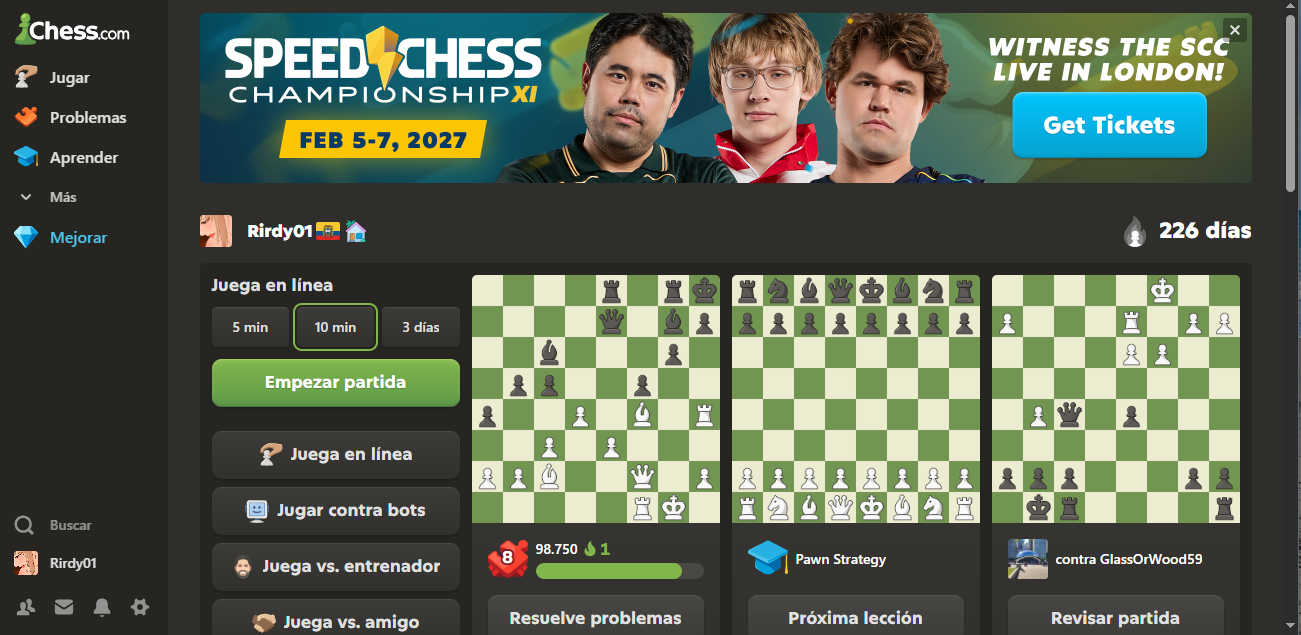
\includegraphics[width=0.85\textwidth]{chess1}
    \caption{Vista principal de la plataforma Chess.com.}
    \label{fig:chess1}
\end{figure}

\begin{figure}[htbp]
    \centering
    
\includegraphics[width=0.85\textwidth]{chess2}
    \caption{Vista del tablero de ajedrez en Chess.com.}
    \label{fig:chess2}
\end{figure}

\begin{figure}[htbp]
    \centering
    
\includegraphics[width=0.85\textwidth]{chess3}
    \caption{Otra funcionalidad de la plataforma Chess.com.}
    \label{fig:chess3}
\end{figure}

\newpage
\section{Tabla de clasificación y criterios de aceptación}

La tabla resume los quince requisitos, su clasificación y la condición que se utilizará para decidir si cada uno cumple. Los criterios se formulan para que puedan comprobarse mediante pruebas, inspecciones o revisión de registros.

\small
\begin{longtable}{p{1.35cm}p{2.35cm}p{5.1cm}p{6cm}}
\caption{Clasificación y criterios de aceptación de los requisitos.}
\label{tab:requisitos}\\
\toprule
\textbf{ID} & \textbf{Tipo} & \textbf{Descripción} & \textbf{Criterio de aceptación}\\
\midrule
\endfirsthead
\toprule
\textbf{ID} & \textbf{Tipo} & \textbf{Descripción} & \textbf{Criterio de aceptación}\\
\midrule
\endhead
RNF-01 & Calidad: desempeño & Propagación del movimiento & En la prueba definida, el percentil 95 del tiempo entre envío y representación es $\leq 150$ ms.\\
RNF-02 & Calidad: fiabilidad & Recuperación de partida & Tras recuperar la conexión, el estado de la partida se restaura en un máximo de 30 segundos.\\
RNF-03 & Calidad: interacción & Contraste visual & Las pantallas principales cumplen una relación de contraste $\geq 4.5:1$ para texto normal.\\
RNF-04 & Calidad: compatibilidad & Navegadores web & El 100\% de los casos críticos se aprueba en cada navegador incluido en el plan de pruebas.\\
RNF-05 & Calidad: mantenibilidad & Complejidad del módulo & El análisis estático muestra una complejidad ciclomática $\leq 12$ por función.\\
RF-01 & Funcional & Emparejamiento & Al solicitar una partida, el sistema asigna un oponente disponible que cumple el rango configurado o informa que no hay uno disponible.\\
RF-02 & Funcional & Actualización de puntuación & Al finalizar la partida, las puntuaciones de ambos jugadores se calculan y registran según el método configurado.\\
RF-03 & Funcional & Exportación PGN & El archivo exportado se genera en formato PGN y conserva la secuencia de movimientos de la partida.\\
RF-04 & Funcional & Historial y reproducción & El usuario puede consultar sus partidas anteriores y reproducir todos los movimientos de una partida seleccionada.\\
RSEG-01 & Seguridad & Protección de contraseñas & La inspección de almacenamiento confirma que no existen contraseñas en texto plano y que se utiliza derivación de claves con sal individual.\\
RSEG-02 & Seguridad & Permisos de moderación & Una cuenta sin rol de moderador no puede ejecutar las funciones restringidas; una cuenta autorizada sí puede hacerlo.\\
RINT-01 & Interfaz & Movimiento táctil & En un dispositivo táctil, el usuario puede seleccionar una pieza y realizar un movimiento legal mediante interacción táctil.\\
RINT-02 & Interfaz & Diseño adaptable & A 360 píxeles de anchura no existe superposición que impida utilizar el tablero o los controles esenciales.\\
RCONF-01 & Confiabilidad & Disponibilidad & Los registros del periodo mensual muestran una disponibilidad del servicio de partidas $\geq 99.5\%$, según la fórmula acordada.\\
RCONF-02 & Confiabilidad & Persistencia de movimientos & Después de una interrupción simulada, el sistema recupera el último movimiento válido confirmado sin alterar la secuencia registrada.\\
\bottomrule
\end{longtable}
\normalsize

\newpage
\section{Autoevaluación y versión corregida de los requisitos}

Para revisar la calidad de los requisitos se identificaron posibles problemas en una primera redacción y se propuso una versión corregida. La autoevaluación considera principalmente claridad, singularidad, completitud y posibilidad de verificación. En los casos en que el requisito ya estaba redactado de manera precisa, se señala qué aspecto se comprobó y se conserva o ajusta su formulación.

\begin{enumerate}[leftmargin=*]
    \item \textbf{RNF-01 -- Desempeño.}\\
    \textit{Primera versión:} ``El tablero debe mostrar las jugadas muy rápido''.\\
    \textbf{Autoevaluación:} la expresión ``muy rápido'' es subjetiva y no establece cómo medir el tiempo de respuesta.\\
    \textbf{Versión corregida:} el sistema debe reflejar en el tablero del oponente un movimiento válido recibido desde el cliente emisor en un máximo de 150 milisegundos, medidos desde el envío del evento hasta su representación en el cliente receptor, bajo una conexión de prueba estable.

    \item \textbf{RNF-02 -- Recuperación.}\\
    \textit{Primera versión:} ``La plataforma debe recuperar la partida rápidamente si se cae el internet''.\\
    \textbf{Autoevaluación:} no define qué significa ``rápidamente'' ni qué estado debe recuperarse.\\
    \textbf{Versión corregida:} cuando un jugador pierda temporalmente la conexión durante una partida, el sistema debe permitirle reconectarse y recuperar el estado de la partida en un máximo de 30 segundos, siempre que la partida continúe activa.

    \item \textbf{RNF-03 -- Accesibilidad.}\\
    \textit{Primera versión:} ``Los colores del tablero deben ser fáciles de distinguir''.\\
    \textbf{Autoevaluación:} ``fáciles de distinguir'' depende de la percepción de cada usuario y no establece un parámetro comprobable.\\
    \textbf{Versión corregida:} la interfaz debe presentar una relación de contraste mínima de 4.5:1 entre el texto normal y su fondo en las pantallas principales de navegación, de acuerdo con el nivel AA de WCAG 2.1.

    \item \textbf{RNF-04 -- Compatibilidad.}\\
    \textit{Primera versión:} ``La página debe funcionar en todos los navegadores''.\\
    \textbf{Autoevaluación:} ``todos'' es una condición demasiado amplia y no identifica los navegadores ni las funciones que se comprobarán.\\
    \textbf{Versión corregida:} la aplicación web debe permitir iniciar sesión, buscar una partida y realizar movimientos legales en las versiones estables de Chrome, Firefox, Safari y Edge incluidas en el plan de pruebas.

    \item \textbf{RNF-05 -- Mantenibilidad.}\\
    \textit{Primera versión:} ``El código del análisis debe ser sencillo de mantener''.\\
    \textbf{Autoevaluación:} ``sencillo'' no tiene un significado medible y no indica qué parte del código se evaluará.\\
    \textbf{Versión corregida:} cada función del módulo de análisis de partidas debe mantener una complejidad ciclomática igual o inferior a 12, según el análisis estático del código.

    \item \textbf{RF-01 -- Emparejamiento.}\\
    \textit{Primera versión:} ``El sistema debe buscar jugadores adecuados para cada usuario''.\\
    \textbf{Autoevaluación:} ``adecuados'' no define las condiciones para seleccionar un oponente.\\
    \textbf{Versión corregida:} el sistema debe asignar un oponente a un usuario que solicite una partida clasificatoria, siempre que exista un jugador disponible dentro del rango de puntuación definido para la modalidad.

    \item \textbf{RF-02 -- Actualización de puntuación.}\\
    \textit{Primera versión:} ``El sistema debe actualizar los puntos de los jugadores al terminar''.\\
    \textbf{Autoevaluación:} no especifica qué puntuaciones se actualizan ni con qué regla se calculan.\\
    \textbf{Versión corregida:} al finalizar una partida clasificatoria, el sistema debe calcular y registrar la nueva puntuación de ambos jugadores de acuerdo con el método de clasificación configurado.

    \item \textbf{RF-03 -- Exportación PGN.}\\
    \textit{Primera versión:} ``El usuario debe poder descargar su partida''.\\
    \textbf{Autoevaluación:} no indica el formato del archivo ni qué información debe contener.\\
    \textbf{Versión corregida:} el sistema debe permitir al usuario exportar los movimientos de una partida finalizada en un archivo con formato PGN.

    \item \textbf{RF-04 -- Historial.}\\
    \textit{Primera versión:} ``El usuario puede revisar sus partidas cuando quiera''.\\
    \textbf{Autoevaluación:} ``cuando quiera'' no define la función y tampoco aclara qué información se presenta.\\
    \textbf{Versión corregida:} el sistema debe mostrar al usuario una lista de sus partidas anteriores y permitir seleccionar una para reproducir sus movimientos.

    \item \textbf{RSEG-01 -- Protección de credenciales.}\\
    \textit{Primera versión:} ``Las contraseñas deben guardarse de forma segura''.\\
    \textbf{Autoevaluación:} ``segura'' es ambiguo y no establece un mecanismo que pueda inspeccionarse.\\
    \textbf{Versión corregida:} el sistema debe almacenar las contraseñas de los usuarios mediante un algoritmo de derivación de claves diseñado para contraseñas, con sal individual, sin guardar contraseñas en texto plano.

    \item \textbf{RSEG-02 -- Control de acceso.}\\
    \textit{Primera versión:} ``Solo las personas autorizadas pueden moderar''.\\
    \textbf{Autoevaluación:} no identifica cómo se determina la autorización ni qué función se restringe.\\
    \textbf{Versión corregida:} el sistema debe permitir el acceso a las funciones de moderación únicamente a las cuentas que tengan asignado el rol de moderador.

    \item \textbf{RINT-01 -- Movimiento táctil.}\\
    \textit{Primera versión:} ``El tablero debe ser cómodo para jugar desde el celular''.\\
    \textbf{Autoevaluación:} ``cómodo'' es subjetivo y no describe la interacción requerida.\\
    \textbf{Versión corregida:} la interfaz debe permitir que el usuario seleccione y mueva una pieza del tablero mediante una interacción táctil en dispositivos con pantalla táctil.

    \item \textbf{RINT-02 -- Diseño adaptable.}\\
    \textit{Primera versión:} ``La página debe adaptarse a cualquier pantalla''.\\
    \textbf{Autoevaluación:} no define un rango de visualización ni qué significa que la adaptación sea correcta.\\
    \textbf{Versión corregida:} la interfaz debe reorganizar los elementos de navegación y el tablero para que puedan utilizarse en pantallas con anchuras desde 360 píxeles, sin superposición de controles esenciales.

    \item \textbf{RCONF-01 -- Disponibilidad.}\\
    \textit{Primera versión:} ``Los servidores deben estar disponibles casi todo el tiempo''.\\
    \textbf{Autoevaluación:} ``casi todo el tiempo'' no permite calcular ni comprobar la disponibilidad.\\
    \textbf{Versión corregida:} el servicio de partidas debe mantener una disponibilidad mensual mínima del 99.5\%, excluyendo los periodos de mantenimiento programado comunicados previamente.

    \item \textbf{RCONF-02 -- Persistencia.}\\
    \textit{Primera versión:} ``El sistema debe guardar todas las partidas para no perder información''.\\
    \textbf{Autoevaluación:} no aclara cuándo se guarda un movimiento ni cómo se comprueba su recuperación.\\
    \textbf{Versión corregida:} el sistema debe guardar cada movimiento válido confirmado en la partida, de manera que pueda recuperarse el último estado registrado después de una interrupción del servicio.
\end{enumerate}

\newpage
\section{Reflexión}

Al realizar esta actividad comprendí que redactar requisitos no consiste únicamente en enumerar las funciones que debería tener una aplicación. También implica analizar las necesidades de quienes la utilizan y expresarlas de una manera que pueda entenderse y comprobarse. Al tomar Chess.com como referencia, pude relacionar conceptos de la norma con situaciones concretas, como el emparejamiento de jugadores, la recuperación de una partida cuando se pierde la conexión y la consulta del historial.

Uno de los aspectos que más me llamó la atención fue la importancia de evitar expresiones generales. Palabras como ``rápido'', ``seguro'' o ``fácil'' pueden parecer suficientes cuando se explica una idea, pero no ayudan al equipo de desarrollo a saber exactamente qué debe implementar. Por eso, convertirlas en métricas, condiciones y criterios de aceptación permite reducir las interpretaciones diferentes y facilita las pruebas.

También pude observar que los requisitos deben analizarse como un conjunto. No tendría sentido definir correctamente el funcionamiento de una partida si no se consideran aspectos como la seguridad, la disponibilidad o la compatibilidad con los dispositivos. En conclusión, la norma ISO/IEC/IEEE 29148:2018 ofrece una guía para organizar las necesidades de un sistema y convertirlas en una base clara para su desarrollo. Aplicarla permite anticipar errores de comunicación y comprobar de manera más objetiva si el producto responde a lo que necesitan sus usuarios.

\begin{thebibliography}{9}
    \bibitem{ieee29148}
    ISO/IEC/IEEE, \emph{Systems and software engineering -- Life cycle processes -- Requirements engineering}, ISO/IEC/IEEE 29148:2018, 2018.

    \bibitem{iso25010}
    ISO/IEC, \emph{Systems and software Quality Requirements and Evaluation (SQuaRE) -- Product quality model}, ISO/IEC 25010:2023, 2023.

    \bibitem{wcag}
    World Wide Web Consortium (W3C), \emph{Web Content Accessibility Guidelines (WCAG) 2.1}, 2018.
\end{thebibliography}

\end{document}
